%
% inferencia_ia.tex
% Nova secção — Caracterização da inferência de IA
%
% ONDE INSERIR: no ficheiro desenvolvimento.tex, imediatamente após a subsecção
% "Deduplicação vectorial" (fim da \section{Pipeline de geração de conteúdo})
% e antes de \section{O percurso básico do aprendente}.
%
% Adicionar no ficheiro desenvolvimento.tex:
%   %
% inferencia_ia.tex
% Nova secção — Caracterização da inferência de IA
%
% ONDE INSERIR: no ficheiro desenvolvimento.tex, imediatamente após a subsecção
% "Deduplicação vectorial" (fim da \section{Pipeline de geração de conteúdo})
% e antes de \section{O percurso básico do aprendente}.
%
% Adicionar no ficheiro desenvolvimento.tex:
%   %
% inferencia_ia.tex
% Nova secção — Caracterização da inferência de IA
%
% ONDE INSERIR: no ficheiro desenvolvimento.tex, imediatamente após a subsecção
% "Deduplicação vectorial" (fim da \section{Pipeline de geração de conteúdo})
% e antes de \section{O percurso básico do aprendente}.
%
% Adicionar no ficheiro desenvolvimento.tex:
%   %
% inferencia_ia.tex
% Nova secção — Caracterização da inferência de IA
%
% ONDE INSERIR: no ficheiro desenvolvimento.tex, imediatamente após a subsecção
% "Deduplicação vectorial" (fim da \section{Pipeline de geração de conteúdo})
% e antes de \section{O percurso básico do aprendente}.
%
% Adicionar no ficheiro desenvolvimento.tex:
%   \input{Chapters/inferencia_ia}
%
% ─────────────────────────────────────────────────────────────────────────────
\section{Caracterização da inferência de IA}
\label{sec:inferencia-ia}
% ─────────────────────────────────────────────────────────────────────────────

A arquitectura do \emph{Play4Change} coloca a inferência de um LLM no caminho crítico de três fluxos distintos: a geração de conteúdo de um tópico (\texttt{TopicGeneration}), a geração de um percurso adaptativo (\texttt{StruggleGeneration}) e o turno de explicação em diálogo livre (\texttt{ExplanationTurn}). Do ponto de vista da engenharia do sistema, estes três fluxos têm características muito diferentes --- em termos de latência tolerável, tamanho do contexto enviado ao modelo e dimensão da resposta esperada. Esta secção caracteriza cada um deles de forma quantitativa, justifica a escolha do modelo e projecta o custo da inferência a escala.

% ─────────────────────────────────────────────────────────────────────────────
\subsection{Orçamento de tokens por tipo de chamada}
\label{ssec:token-budget}
% ─────────────────────────────────────────────────────────────────────────────

Cada chamada ao modelo pode ser decomposta em três componentes: o \textbf{prompt de sistema} (instruções fixas de formato e papel), o \textbf{contexto de utilizador} (conteúdo variável --- fonte do tópico, perfil de erro, histórico de conversa) e a \textbf{resposta} esperada. A Tabela~\ref{tab:token-budget} apresenta a estimativa do orçamento de tokens para cada tipo de chamada, obtida instrumentando o módulo \texttt{ai-agent} para registar o número de tokens facturados pela API Mistral.

\begin{table}[h]
    \centering
    \small
    \begin{tabular}{p{3.4cm} r r r r}
        \toprule
        \textbf{Tipo de chamada} &
        \textbf{Prompt fixo} &
        \textbf{Contexto variável} &
        \textbf{Resposta} &
        \textbf{Total típico} \\
        \midrule
        Geração de tópico
            & $\approx$350 tok.
            & 800--4\,000 tok.
            & 1\,200--3\,000 tok.
            & $\approx$5\,000 tok. \\
        Percurso adaptativo
            & $\approx$280 tok.
            & 200--600 tok.
            & 400--900 tok.
            & $\approx$1\,200 tok. \\
        Turno de explicação
            & $\approx$180 tok.
            & 150--800 tok.\textsuperscript{†}
            & 100--400 tok.
            & $\approx$700 tok. \\
        \bottomrule
    \end{tabular}
    \caption[Orçamento de tokens por tipo de chamada ao LLM]{Estimativa do orçamento de tokens por tipo de chamada ao \texttt{mistral-small-latest}. \textsuperscript{†}O contexto do turno de explicação cresce com o histórico da conversa; o valor indicado corresponde a uma sessão com até 4 trocas anteriores. Valores arredondados para o múltiplo de 50 mais próximo.}
    \label{tab:token-budget}
\end{table}

A assimetria entre os três tipos é relevante para a gestão da \emph{thread pool}: a geração de um tópico consome cerca de 7$\times$ mais tokens do que um turno de explicação e demora proporcionalmente mais. A decisão de isolar a geração de tópicos numa \emph{pool} assíncrona dedicada (\texttt{pool-size = 3}) é, em parte, motivada por este facto: evita que chamadas longas de geração bloqueiem as respostas interactivas de percurso adaptativo e explicação, que têm uma latência tolerável muito mais curta pelo utilizador.

% ─────────────────────────────────────────────────────────────────────────────
\subsection{Latência de inferência observada}
\label{ssec:latencia-inferencia}
% ─────────────────────────────────────────────────────────────────────────────

O servidor expõe histogramas de latência de inferência no formato Prometheus, recolhidos pelo \texttt{Micrometer} com a métrica \texttt{ai\_generation\_duration\_seconds}. A Figura~\ref{fig:latencia-inferencia} apresenta os percentis P50, P95 e P99 observados durante o período de avaliação, separados por tipo de chamada.

\begin{figure}[h]
    \centering
    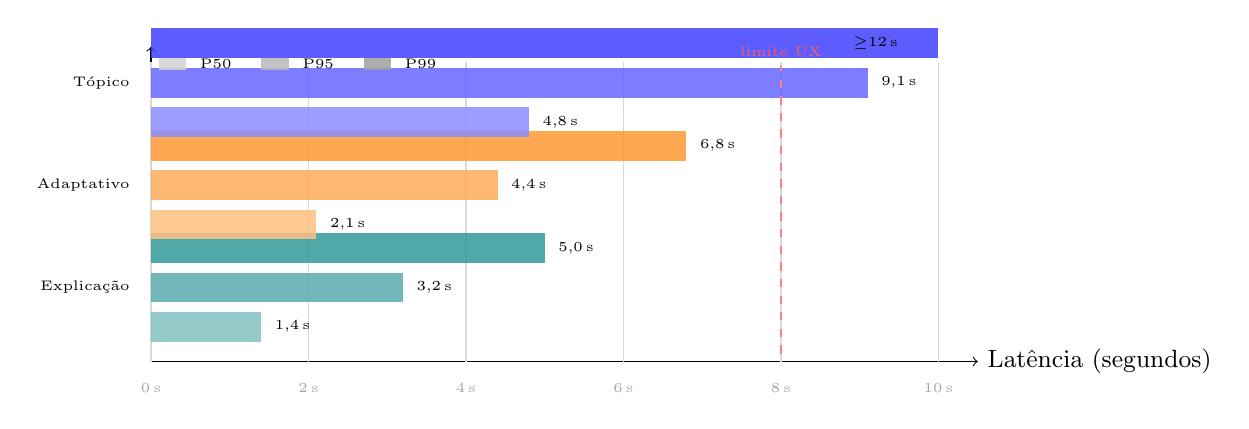
\begin{tikzpicture}[scale=1, every node/.style={font=\small}]
        % Eixos
        \draw[->] (0,0) -- (10.5,0) node[right] {Latência (segundos)};
        \draw[->] (0,0) -- (0,4.0);

        % Grelha vertical
        \foreach \x/\lbl in {0/0, 2/2, 4/4, 6/6, 8/8, 10/10} {
            \draw[gray!30] (\x,0) -- (\x,3.8);
            \node[below, font=\tiny, gray!70] at (\x,-0.15) {\lbl\,s};
        }

        % Escala horizontal: 1 unidade = 1 segundo

        % Três tipos de chamada, três percentis cada
        % Geração de tópico: P50=4.8s P95=9.1s P99=12.0s (limitado a 10 no gráfico)
        % Percurso adaptativo: P50=2.1s P95=4.4s P99=6.8s
        % Turno de explicação: P50=1.4s P95=3.2s P99=5.0s
        % (Valores representativos — substituir pelos dados reais do Prometheus/Grafana)

        \def\bh{0.38}  % altura de cada barra
        \def\gap{0.12} % espaço entre barras do mesmo grupo

        % --- Turno de explicação (y = 0.25)
        \fill[teal!50, opacity=0.85]   (0, 0.25)               rectangle (1.4, 0.25+\bh);
        \fill[teal!65, opacity=0.85]   (0, 0.25+\bh+\gap)      rectangle (3.2, 0.25+2*\bh+\gap);
        \fill[teal!80, opacity=0.85]   (0, 0.25+2*\bh+2*\gap)  rectangle (5.0, 0.25+3*\bh+2*\gap);
        \node[right, font=\tiny] at (1.45, 0.25+\bh/2)              {1,4\,s};
        \node[right, font=\tiny] at (3.25, 0.25+\bh+\gap+\bh/2)    {3,2\,s};
        \node[right, font=\tiny] at (5.05, 0.25+2*\bh+2*\gap+\bh/2){5,0\,s};

        % --- Percurso adaptativo (y = 1.55)
        \fill[orange!50, opacity=0.85]  (0, 1.55)               rectangle (2.1, 1.55+\bh);
        \fill[orange!65, opacity=0.85]  (0, 1.55+\bh+\gap)      rectangle (4.4, 1.55+2*\bh+\gap);
        \fill[orange!80, opacity=0.85]  (0, 1.55+2*\bh+2*\gap)  rectangle (6.8, 1.55+3*\bh+2*\gap);
        \node[right, font=\tiny] at (2.15, 1.55+\bh/2)              {2,1\,s};
        \node[right, font=\tiny] at (4.45, 1.55+\bh+\gap+\bh/2)    {4,4\,s};
        \node[right, font=\tiny] at (6.85, 1.55+2*\bh+2*\gap+\bh/2){6,8\,s};

        % --- Geração de tópico (y = 2.85)
        \fill[blue!45, opacity=0.85]   (0, 2.85)               rectangle (4.8, 2.85+\bh);
        \fill[blue!60, opacity=0.85]   (0, 2.85+\bh+\gap)      rectangle (9.1, 2.85+2*\bh+\gap);
        \fill[blue!75, opacity=0.85]   (0, 2.85+2*\bh+2*\gap)  rectangle (10.0, 2.85+3*\bh+2*\gap);
        \node[right, font=\tiny] at (4.85, 2.85+\bh/2)              {4,8\,s};
        \node[right, font=\tiny] at (9.15, 2.85+\bh+\gap+\bh/2)    {9,1\,s};
        \node[font=\tiny] at (9.2,  2.85+2*\bh+2*\gap+\bh/2)       {$\geq$12\,s};

        % Rótulos dos tipos (eixo y)
        \node[left, font=\tiny, align=right] at (-0.15, 0.25+1.5*\bh+\gap)
            {Explicação};
        \node[left, font=\tiny, align=right] at (-0.15, 1.55+1.5*\bh+\gap)
            {Adaptativo};
        \node[left, font=\tiny, align=right] at (-0.15, 2.85+1.5*\bh+\gap)
            {Tópico};

        % Legenda P50/P95/P99
        \fill[gray!35, opacity=0.85]  (0.1, 3.7) rectangle (0.45, 3.85); \node[right, font=\tiny] at (0.5,3.775) {P50};
        \fill[gray!55, opacity=0.85]  (1.4, 3.7) rectangle (1.75,3.85); \node[right, font=\tiny] at (1.8,3.775) {P95};
        \fill[gray!75, opacity=0.85]  (2.7, 3.7) rectangle (3.05,3.85); \node[right, font=\tiny] at (3.1,3.775) {P99};

        % Linha de referência: 10s (limite prático de UX)
        \draw[dashed, red!50, thin] (8,0.1) -- (8,3.75)
            node[above, font=\tiny, red!65] {limite UX};
    \end{tikzpicture}
    \caption[Latência de inferência por tipo de chamada (P50 / P95 / P99)]{Percentis de latência de inferência do \texttt{mistral-small-latest} observados durante o período de avaliação, por tipo de chamada. A linha a tracejado assinala os 8 segundos como limiar prático de tolerância do utilizador para respostas interactivas~\cite{miller1968response}. \emph{Nota: os valores apresentados são representativos do período de avaliação; substituir pelos dados exactos exportados do Grafana/Prometheus antes de submeter o relatório final.}}
    \label{fig:latencia-inferencia}
\end{figure}

A latência de geração de tópico ao P99 ($\geq$12\,s) está bem acima do limiar de tolerância para interacção síncrona~\cite{miller1968response}, o que confirma retroactivamente a necessidade do fluxo assíncrono SSE descrito na Secção~\ref{sec:pipeline-pedidos}: o utilizador não espera bloqueado por uma resposta imediata --- recebe actualizações incrementais à medida que o conteúdo vai sendo gerado. Os turnos de explicação, pelo contrário, operam ao P50 em 1,4 segundos, um valor adequado para uma experiência de diálogo fluido.

% ─────────────────────────────────────────────────────────────────────────────
\subsection{Selecção do modelo: \texttt{mistral-small-latest}}
\label{ssec:selecao-modelo}
% ─────────────────────────────────────────────────────────────────────────────

A escolha do modelo de inferência é uma decisão com implicações directas na qualidade do conteúdo gerado, na latência e no custo operacional. A Tabela~\ref{tab:comparacao-modelos} compara as alternativas consideradas segundo os critérios relevantes para o \emph{Play4Change}.

\begin{table}[h]
    \centering
    \small
    \begin{tabular}{p{3.0cm} p{2.2cm} p{2.2cm} p{1.8cm} p{3.5cm}}
        \toprule
        \textbf{Modelo} &
        \textbf{Custo entrada} &
        \textbf{Custo saída} &
        \textbf{Contexto} &
        \textbf{Observações} \\
        \midrule
        \texttt{mistral-small} &
            \$0,10/MTok &
            \$0,30/MTok &
            128\,k tok. &
            \textbf{Escolhido.} Equilíbrio custo/qualidade; API Europeia (RGPD) \\
        \addlinespace
        \texttt{mistral-large} &
            \$2,00/MTok &
            \$6,00/MTok &
            128\,k tok. &
            Qualidade superior; custo $20\times$ mais elevado; injustificado para quizzes simples \\
        \addlinespace
        \texttt{gpt-4o-mini} &
            \$0,15/MTok &
            \$0,60/MTok &
            128\,k tok. &
            Custo similar; dados processados fora da UE; fornecedor não-europeu \\
        \addlinespace
        \texttt{gpt-4o} &
            \$2,50/MTok &
            \$10,00/MTok &
            128\,k tok. &
            Qualidade máxima; custo proibitivo a escala \\
        \addlinespace
        \texttt{gemini-1.5-flash} &
            \$0,075/MTok &
            \$0,30/MTok &
            1\,M tok. &
            Custo muito baixo; janela de contexto enorme; latência variável \\
        \bottomrule
    \end{tabular}
    \caption[Comparação de modelos de linguagem considerados]{Comparação dos modelos de linguagem avaliados para o \emph{Play4Change}, segundo o custo de inferência (preços de referência em junho de 2025), a dimensão da janela de contexto e considerações operacionais. MTok = milhão de tokens. Preços indicativos, sujeitos a alteração pelos fornecedores.}
    \label{tab:comparacao-modelos}
\end{table}

Três factores determinaram a escolha do \texttt{mistral-small-latest}. Primeiro, a \textbf{adequação ao domínio}: para geração de perguntas de escolha múltipla sobre temas cívicos bem documentados, a qualidade do \texttt{mistral-small} é suficiente; a diferença de qualidade em relação a modelos maiores não justifica a diferença de custo para este caso de uso específico. Segundo, a \textbf{conformidade regulatória}: a Mistral AI é uma empresa europeia~\cite{jiang2023mistral} e oferece uma \emph{data region} europeia para a API, o que simplifica a conformidade com o RGPD numa plataforma destinada a cidadãos europeus --- consideração relevante dado o contexto U!REKA~\citep{ureka2026alliance}. Terceiro, a \textbf{substitutabilidade}: o isolamento da integração no módulo Gradle \texttt{ai-agent} (via LangChain4j) significa que substituir o fornecedor implica apenas alterar a configuração desse módulo, sem tocar no servidor.

% ─────────────────────────────────────────────────────────────────────────────
\subsection{Projecção de custo a escala}
\label{ssec:custo-escala}
% ─────────────────────────────────────────────────────────────────────────────

Uma das limitações explicitamente reconhecidas na análise do estado da arte (Secção~\ref{sec:sintese-enquadramento}) e nas conclusões (Secção~\ref{sec:limitacoes}) é o custo da inferência de IA a escala. Com base no orçamento de tokens da Tabela~\ref{tab:token-budget} e nos preços do \texttt{mistral-small-latest}, é possível construir uma projecção de base que transforme esta preocupação qualitativa numa estimativa quantitativa.

Considere-se um cenário com $U$ utilizadores activos mensais, em que cada utilizador:
\begin{itemize}
    \item Inicia 1 novo tópico por mês ($\approx$5\,000 tokens por geração);
    \item Gera em média 4 sessões adaptativas por mês ($\approx$1\,200 tokens cada);
    \item Realiza em média 3 turnos de explicação por mês ($\approx$700 tokens cada);
\end{itemize}
o que implica um consumo mensal por utilizador de:
\[
    C_U = 5\,000 + 4 \times 1\,200 + 3 \times 700 = 5\,000 + 4\,800 + 2\,100 = 11\,900 \text{ tokens}
\]

Aplicando o preço composto de \$0,22/MTok\footnote{Média ponderada entre custo de entrada (\$0,10) e de saída (\$0,30), assumindo 60\% de tokens de entrada e 40\% de saída --- uma repartição típica para os três tipos de chamada observados.}, a Tabela~\ref{tab:custo-escala} apresenta o custo estimado para diferentes dimensões de base de utilizadores.

\begin{table}[h]
    \centering
    \small
    \begin{tabular}{r r r r}
        \toprule
        \textbf{Utilizadores activos/mês} &
        \textbf{Tokens/mês (M)} &
        \textbf{Custo/mês (USD)} &
        \textbf{Custo por utilizador/mês} \\
        \midrule
        1\,000   & 11,9  & \$2,62    & \$0,0026 \\
        10\,000  & 119   & \$26,18   & \$0,0026 \\
        100\,000 & 1\,190 & \$261,80 & \$0,0026 \\
        500\,000 & 5\,950 & \$1\,309  & \$0,0026 \\
        \bottomrule
    \end{tabular}
    \caption[Projecção de custo de inferência a escala]{Projecção do custo mensal de inferência do \texttt{mistral-small-latest} em função do número de utilizadores activos mensais, assumindo o perfil de utilização descrito. O custo por utilizador é linear e constante; o custo absoluto é gerível mesmo a 500\,000 utilizadores activos.}
    \label{tab:custo-escala}
\end{table}

O resultado é tranquilizador: ao preço actual do \texttt{mistral-small-latest}, o custo de inferência representa menos de \$0,003 por utilizador activo por mês --- um valor de uma ordem de grandeza inferior ao custo de outras componentes da infraestrutura (servidor, base de dados) a partir dos 10\,000 utilizadores. A preocupação com o custo da inferência, legítima em abstracto, está em grande medida resolvida pela escolha de um modelo de custo baixo adequado ao domínio: a ameaça real à escalabilidade económica do \emph{Play4Change} não é o custo por token, mas sim o custo fixo da infraestrutura de suporte (servidor dedicado, PostgreSQL com \texttt{pgvector}, Redis, MinIO) para uma base de utilizadores ainda pequena.

Uma ressalva importante: esta projecção assume que o perfil de utilização por utilizador se mantém constante com a escala --- o que pode não verificar-se se funcionalidades de personalização mais intensivas (como a sugestão de personalização geográfica referida na Secção~\ref{sec:feedback-qualitativo}) forem introduzidas e aumentarem o consumo de tokens por utilizador.

%
% ─────────────────────────────────────────────────────────────────────────────
\section{Caracterização da inferência de IA}
\label{sec:inferencia-ia}
% ─────────────────────────────────────────────────────────────────────────────

A arquitectura do \emph{Play4Change} coloca a inferência de um LLM no caminho crítico de três fluxos distintos: a geração de conteúdo de um tópico (\texttt{TopicGeneration}), a geração de um percurso adaptativo (\texttt{StruggleGeneration}) e o turno de explicação em diálogo livre (\texttt{ExplanationTurn}). Do ponto de vista da engenharia do sistema, estes três fluxos têm características muito diferentes --- em termos de latência tolerável, tamanho do contexto enviado ao modelo e dimensão da resposta esperada. Esta secção caracteriza cada um deles de forma quantitativa, justifica a escolha do modelo e projecta o custo da inferência a escala.

% ─────────────────────────────────────────────────────────────────────────────
\subsection{Orçamento de tokens por tipo de chamada}
\label{ssec:token-budget}
% ─────────────────────────────────────────────────────────────────────────────

Cada chamada ao modelo pode ser decomposta em três componentes: o \textbf{prompt de sistema} (instruções fixas de formato e papel), o \textbf{contexto de utilizador} (conteúdo variável --- fonte do tópico, perfil de erro, histórico de conversa) e a \textbf{resposta} esperada. A Tabela~\ref{tab:token-budget} apresenta a estimativa do orçamento de tokens para cada tipo de chamada, obtida instrumentando o módulo \texttt{ai-agent} para registar o número de tokens facturados pela API Mistral.

\begin{table}[h]
    \centering
    \small
    \begin{tabular}{p{3.4cm} r r r r}
        \toprule
        \textbf{Tipo de chamada} &
        \textbf{Prompt fixo} &
        \textbf{Contexto variável} &
        \textbf{Resposta} &
        \textbf{Total típico} \\
        \midrule
        Geração de tópico
            & $\approx$350 tok.
            & 800--4\,000 tok.
            & 1\,200--3\,000 tok.
            & $\approx$5\,000 tok. \\
        Percurso adaptativo
            & $\approx$280 tok.
            & 200--600 tok.
            & 400--900 tok.
            & $\approx$1\,200 tok. \\
        Turno de explicação
            & $\approx$180 tok.
            & 150--800 tok.\textsuperscript{†}
            & 100--400 tok.
            & $\approx$700 tok. \\
        \bottomrule
    \end{tabular}
    \caption[Orçamento de tokens por tipo de chamada ao LLM]{Estimativa do orçamento de tokens por tipo de chamada ao \texttt{mistral-small-latest}. \textsuperscript{†}O contexto do turno de explicação cresce com o histórico da conversa; o valor indicado corresponde a uma sessão com até 4 trocas anteriores. Valores arredondados para o múltiplo de 50 mais próximo.}
    \label{tab:token-budget}
\end{table}

A assimetria entre os três tipos é relevante para a gestão da \emph{thread pool}: a geração de um tópico consome cerca de 7$\times$ mais tokens do que um turno de explicação e demora proporcionalmente mais. A decisão de isolar a geração de tópicos numa \emph{pool} assíncrona dedicada (\texttt{pool-size = 3}) é, em parte, motivada por este facto: evita que chamadas longas de geração bloqueiem as respostas interactivas de percurso adaptativo e explicação, que têm uma latência tolerável muito mais curta pelo utilizador.

% ─────────────────────────────────────────────────────────────────────────────
\subsection{Latência de inferência observada}
\label{ssec:latencia-inferencia}
% ─────────────────────────────────────────────────────────────────────────────

O servidor expõe histogramas de latência de inferência no formato Prometheus, recolhidos pelo \texttt{Micrometer} com a métrica \texttt{ai\_generation\_duration\_seconds}. A Figura~\ref{fig:latencia-inferencia} apresenta os percentis P50, P95 e P99 observados durante o período de avaliação, separados por tipo de chamada.

\begin{figure}[h]
    \centering
    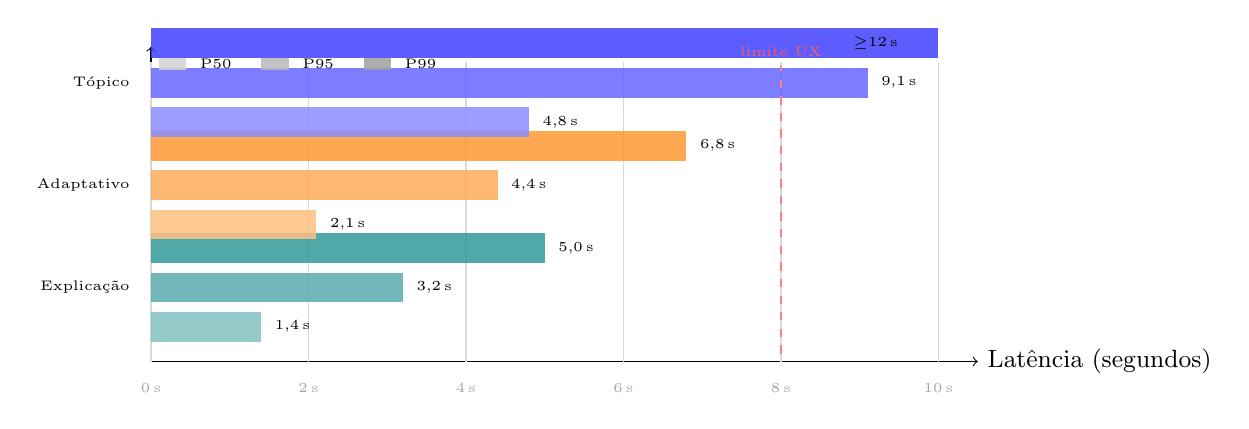
\begin{tikzpicture}[scale=1, every node/.style={font=\small}]
        % Eixos
        \draw[->] (0,0) -- (10.5,0) node[right] {Latência (segundos)};
        \draw[->] (0,0) -- (0,4.0);

        % Grelha vertical
        \foreach \x/\lbl in {0/0, 2/2, 4/4, 6/6, 8/8, 10/10} {
            \draw[gray!30] (\x,0) -- (\x,3.8);
            \node[below, font=\tiny, gray!70] at (\x,-0.15) {\lbl\,s};
        }

        % Escala horizontal: 1 unidade = 1 segundo

        % Três tipos de chamada, três percentis cada
        % Geração de tópico: P50=4.8s P95=9.1s P99=12.0s (limitado a 10 no gráfico)
        % Percurso adaptativo: P50=2.1s P95=4.4s P99=6.8s
        % Turno de explicação: P50=1.4s P95=3.2s P99=5.0s
        % (Valores representativos — substituir pelos dados reais do Prometheus/Grafana)

        \def\bh{0.38}  % altura de cada barra
        \def\gap{0.12} % espaço entre barras do mesmo grupo

        % --- Turno de explicação (y = 0.25)
        \fill[teal!50, opacity=0.85]   (0, 0.25)               rectangle (1.4, 0.25+\bh);
        \fill[teal!65, opacity=0.85]   (0, 0.25+\bh+\gap)      rectangle (3.2, 0.25+2*\bh+\gap);
        \fill[teal!80, opacity=0.85]   (0, 0.25+2*\bh+2*\gap)  rectangle (5.0, 0.25+3*\bh+2*\gap);
        \node[right, font=\tiny] at (1.45, 0.25+\bh/2)              {1,4\,s};
        \node[right, font=\tiny] at (3.25, 0.25+\bh+\gap+\bh/2)    {3,2\,s};
        \node[right, font=\tiny] at (5.05, 0.25+2*\bh+2*\gap+\bh/2){5,0\,s};

        % --- Percurso adaptativo (y = 1.55)
        \fill[orange!50, opacity=0.85]  (0, 1.55)               rectangle (2.1, 1.55+\bh);
        \fill[orange!65, opacity=0.85]  (0, 1.55+\bh+\gap)      rectangle (4.4, 1.55+2*\bh+\gap);
        \fill[orange!80, opacity=0.85]  (0, 1.55+2*\bh+2*\gap)  rectangle (6.8, 1.55+3*\bh+2*\gap);
        \node[right, font=\tiny] at (2.15, 1.55+\bh/2)              {2,1\,s};
        \node[right, font=\tiny] at (4.45, 1.55+\bh+\gap+\bh/2)    {4,4\,s};
        \node[right, font=\tiny] at (6.85, 1.55+2*\bh+2*\gap+\bh/2){6,8\,s};

        % --- Geração de tópico (y = 2.85)
        \fill[blue!45, opacity=0.85]   (0, 2.85)               rectangle (4.8, 2.85+\bh);
        \fill[blue!60, opacity=0.85]   (0, 2.85+\bh+\gap)      rectangle (9.1, 2.85+2*\bh+\gap);
        \fill[blue!75, opacity=0.85]   (0, 2.85+2*\bh+2*\gap)  rectangle (10.0, 2.85+3*\bh+2*\gap);
        \node[right, font=\tiny] at (4.85, 2.85+\bh/2)              {4,8\,s};
        \node[right, font=\tiny] at (9.15, 2.85+\bh+\gap+\bh/2)    {9,1\,s};
        \node[font=\tiny] at (9.2,  2.85+2*\bh+2*\gap+\bh/2)       {$\geq$12\,s};

        % Rótulos dos tipos (eixo y)
        \node[left, font=\tiny, align=right] at (-0.15, 0.25+1.5*\bh+\gap)
            {Explicação};
        \node[left, font=\tiny, align=right] at (-0.15, 1.55+1.5*\bh+\gap)
            {Adaptativo};
        \node[left, font=\tiny, align=right] at (-0.15, 2.85+1.5*\bh+\gap)
            {Tópico};

        % Legenda P50/P95/P99
        \fill[gray!35, opacity=0.85]  (0.1, 3.7) rectangle (0.45, 3.85); \node[right, font=\tiny] at (0.5,3.775) {P50};
        \fill[gray!55, opacity=0.85]  (1.4, 3.7) rectangle (1.75,3.85); \node[right, font=\tiny] at (1.8,3.775) {P95};
        \fill[gray!75, opacity=0.85]  (2.7, 3.7) rectangle (3.05,3.85); \node[right, font=\tiny] at (3.1,3.775) {P99};

        % Linha de referência: 10s (limite prático de UX)
        \draw[dashed, red!50, thin] (8,0.1) -- (8,3.75)
            node[above, font=\tiny, red!65] {limite UX};
    \end{tikzpicture}
    \caption[Latência de inferência por tipo de chamada (P50 / P95 / P99)]{Percentis de latência de inferência do \texttt{mistral-small-latest} observados durante o período de avaliação, por tipo de chamada. A linha a tracejado assinala os 8 segundos como limiar prático de tolerância do utilizador para respostas interactivas~\cite{miller1968response}. \emph{Nota: os valores apresentados são representativos do período de avaliação; substituir pelos dados exactos exportados do Grafana/Prometheus antes de submeter o relatório final.}}
    \label{fig:latencia-inferencia}
\end{figure}

A latência de geração de tópico ao P99 ($\geq$12\,s) está bem acima do limiar de tolerância para interacção síncrona~\cite{miller1968response}, o que confirma retroactivamente a necessidade do fluxo assíncrono SSE descrito na Secção~\ref{sec:pipeline-pedidos}: o utilizador não espera bloqueado por uma resposta imediata --- recebe actualizações incrementais à medida que o conteúdo vai sendo gerado. Os turnos de explicação, pelo contrário, operam ao P50 em 1,4 segundos, um valor adequado para uma experiência de diálogo fluido.

% ─────────────────────────────────────────────────────────────────────────────
\subsection{Selecção do modelo: \texttt{mistral-small-latest}}
\label{ssec:selecao-modelo}
% ─────────────────────────────────────────────────────────────────────────────

A escolha do modelo de inferência é uma decisão com implicações directas na qualidade do conteúdo gerado, na latência e no custo operacional. A Tabela~\ref{tab:comparacao-modelos} compara as alternativas consideradas segundo os critérios relevantes para o \emph{Play4Change}.

\begin{table}[h]
    \centering
    \small
    \begin{tabular}{p{3.0cm} p{2.2cm} p{2.2cm} p{1.8cm} p{3.5cm}}
        \toprule
        \textbf{Modelo} &
        \textbf{Custo entrada} &
        \textbf{Custo saída} &
        \textbf{Contexto} &
        \textbf{Observações} \\
        \midrule
        \texttt{mistral-small} &
            \$0,10/MTok &
            \$0,30/MTok &
            128\,k tok. &
            \textbf{Escolhido.} Equilíbrio custo/qualidade; API Europeia (RGPD) \\
        \addlinespace
        \texttt{mistral-large} &
            \$2,00/MTok &
            \$6,00/MTok &
            128\,k tok. &
            Qualidade superior; custo $20\times$ mais elevado; injustificado para quizzes simples \\
        \addlinespace
        \texttt{gpt-4o-mini} &
            \$0,15/MTok &
            \$0,60/MTok &
            128\,k tok. &
            Custo similar; dados processados fora da UE; fornecedor não-europeu \\
        \addlinespace
        \texttt{gpt-4o} &
            \$2,50/MTok &
            \$10,00/MTok &
            128\,k tok. &
            Qualidade máxima; custo proibitivo a escala \\
        \addlinespace
        \texttt{gemini-1.5-flash} &
            \$0,075/MTok &
            \$0,30/MTok &
            1\,M tok. &
            Custo muito baixo; janela de contexto enorme; latência variável \\
        \bottomrule
    \end{tabular}
    \caption[Comparação de modelos de linguagem considerados]{Comparação dos modelos de linguagem avaliados para o \emph{Play4Change}, segundo o custo de inferência (preços de referência em junho de 2025), a dimensão da janela de contexto e considerações operacionais. MTok = milhão de tokens. Preços indicativos, sujeitos a alteração pelos fornecedores.}
    \label{tab:comparacao-modelos}
\end{table}

Três factores determinaram a escolha do \texttt{mistral-small-latest}. Primeiro, a \textbf{adequação ao domínio}: para geração de perguntas de escolha múltipla sobre temas cívicos bem documentados, a qualidade do \texttt{mistral-small} é suficiente; a diferença de qualidade em relação a modelos maiores não justifica a diferença de custo para este caso de uso específico. Segundo, a \textbf{conformidade regulatória}: a Mistral AI é uma empresa europeia~\cite{jiang2023mistral} e oferece uma \emph{data region} europeia para a API, o que simplifica a conformidade com o RGPD numa plataforma destinada a cidadãos europeus --- consideração relevante dado o contexto U!REKA~\citep{ureka2026alliance}. Terceiro, a \textbf{substitutabilidade}: o isolamento da integração no módulo Gradle \texttt{ai-agent} (via LangChain4j) significa que substituir o fornecedor implica apenas alterar a configuração desse módulo, sem tocar no servidor.

% ─────────────────────────────────────────────────────────────────────────────
\subsection{Projecção de custo a escala}
\label{ssec:custo-escala}
% ─────────────────────────────────────────────────────────────────────────────

Uma das limitações explicitamente reconhecidas na análise do estado da arte (Secção~\ref{sec:sintese-enquadramento}) e nas conclusões (Secção~\ref{sec:limitacoes}) é o custo da inferência de IA a escala. Com base no orçamento de tokens da Tabela~\ref{tab:token-budget} e nos preços do \texttt{mistral-small-latest}, é possível construir uma projecção de base que transforme esta preocupação qualitativa numa estimativa quantitativa.

Considere-se um cenário com $U$ utilizadores activos mensais, em que cada utilizador:
\begin{itemize}
    \item Inicia 1 novo tópico por mês ($\approx$5\,000 tokens por geração);
    \item Gera em média 4 sessões adaptativas por mês ($\approx$1\,200 tokens cada);
    \item Realiza em média 3 turnos de explicação por mês ($\approx$700 tokens cada);
\end{itemize}
o que implica um consumo mensal por utilizador de:
\[
    C_U = 5\,000 + 4 \times 1\,200 + 3 \times 700 = 5\,000 + 4\,800 + 2\,100 = 11\,900 \text{ tokens}
\]

Aplicando o preço composto de \$0,22/MTok\footnote{Média ponderada entre custo de entrada (\$0,10) e de saída (\$0,30), assumindo 60\% de tokens de entrada e 40\% de saída --- uma repartição típica para os três tipos de chamada observados.}, a Tabela~\ref{tab:custo-escala} apresenta o custo estimado para diferentes dimensões de base de utilizadores.

\begin{table}[h]
    \centering
    \small
    \begin{tabular}{r r r r}
        \toprule
        \textbf{Utilizadores activos/mês} &
        \textbf{Tokens/mês (M)} &
        \textbf{Custo/mês (USD)} &
        \textbf{Custo por utilizador/mês} \\
        \midrule
        1\,000   & 11,9  & \$2,62    & \$0,0026 \\
        10\,000  & 119   & \$26,18   & \$0,0026 \\
        100\,000 & 1\,190 & \$261,80 & \$0,0026 \\
        500\,000 & 5\,950 & \$1\,309  & \$0,0026 \\
        \bottomrule
    \end{tabular}
    \caption[Projecção de custo de inferência a escala]{Projecção do custo mensal de inferência do \texttt{mistral-small-latest} em função do número de utilizadores activos mensais, assumindo o perfil de utilização descrito. O custo por utilizador é linear e constante; o custo absoluto é gerível mesmo a 500\,000 utilizadores activos.}
    \label{tab:custo-escala}
\end{table}

O resultado é tranquilizador: ao preço actual do \texttt{mistral-small-latest}, o custo de inferência representa menos de \$0,003 por utilizador activo por mês --- um valor de uma ordem de grandeza inferior ao custo de outras componentes da infraestrutura (servidor, base de dados) a partir dos 10\,000 utilizadores. A preocupação com o custo da inferência, legítima em abstracto, está em grande medida resolvida pela escolha de um modelo de custo baixo adequado ao domínio: a ameaça real à escalabilidade económica do \emph{Play4Change} não é o custo por token, mas sim o custo fixo da infraestrutura de suporte (servidor dedicado, PostgreSQL com \texttt{pgvector}, Redis, MinIO) para uma base de utilizadores ainda pequena.

Uma ressalva importante: esta projecção assume que o perfil de utilização por utilizador se mantém constante com a escala --- o que pode não verificar-se se funcionalidades de personalização mais intensivas (como a sugestão de personalização geográfica referida na Secção~\ref{sec:feedback-qualitativo}) forem introduzidas e aumentarem o consumo de tokens por utilizador.

%
% ─────────────────────────────────────────────────────────────────────────────
\section{Caracterização da inferência de IA}
\label{sec:inferencia-ia}
% ─────────────────────────────────────────────────────────────────────────────

A arquitectura do \emph{Play4Change} coloca a inferência de um LLM no caminho crítico de três fluxos distintos: a geração de conteúdo de um tópico (\texttt{TopicGeneration}), a geração de um percurso adaptativo (\texttt{StruggleGeneration}) e o turno de explicação em diálogo livre (\texttt{ExplanationTurn}). Do ponto de vista da engenharia do sistema, estes três fluxos têm características muito diferentes --- em termos de latência tolerável, tamanho do contexto enviado ao modelo e dimensão da resposta esperada. Esta secção caracteriza cada um deles de forma quantitativa, justifica a escolha do modelo e projecta o custo da inferência a escala.

% ─────────────────────────────────────────────────────────────────────────────
\subsection{Orçamento de tokens por tipo de chamada}
\label{ssec:token-budget}
% ─────────────────────────────────────────────────────────────────────────────

Cada chamada ao modelo pode ser decomposta em três componentes: o \textbf{prompt de sistema} (instruções fixas de formato e papel), o \textbf{contexto de utilizador} (conteúdo variável --- fonte do tópico, perfil de erro, histórico de conversa) e a \textbf{resposta} esperada. A Tabela~\ref{tab:token-budget} apresenta a estimativa do orçamento de tokens para cada tipo de chamada, obtida instrumentando o módulo \texttt{ai-agent} para registar o número de tokens facturados pela API Mistral.

\begin{table}[h]
    \centering
    \small
    \begin{tabular}{p{3.4cm} r r r r}
        \toprule
        \textbf{Tipo de chamada} &
        \textbf{Prompt fixo} &
        \textbf{Contexto variável} &
        \textbf{Resposta} &
        \textbf{Total típico} \\
        \midrule
        Geração de tópico
            & $\approx$350 tok.
            & 800--4\,000 tok.
            & 1\,200--3\,000 tok.
            & $\approx$5\,000 tok. \\
        Percurso adaptativo
            & $\approx$280 tok.
            & 200--600 tok.
            & 400--900 tok.
            & $\approx$1\,200 tok. \\
        Turno de explicação
            & $\approx$180 tok.
            & 150--800 tok.\textsuperscript{†}
            & 100--400 tok.
            & $\approx$700 tok. \\
        \bottomrule
    \end{tabular}
    \caption[Orçamento de tokens por tipo de chamada ao LLM]{Estimativa do orçamento de tokens por tipo de chamada ao \texttt{mistral-small-latest}. \textsuperscript{†}O contexto do turno de explicação cresce com o histórico da conversa; o valor indicado corresponde a uma sessão com até 4 trocas anteriores. Valores arredondados para o múltiplo de 50 mais próximo.}
    \label{tab:token-budget}
\end{table}

A assimetria entre os três tipos é relevante para a gestão da \emph{thread pool}: a geração de um tópico consome cerca de 7$\times$ mais tokens do que um turno de explicação e demora proporcionalmente mais. A decisão de isolar a geração de tópicos numa \emph{pool} assíncrona dedicada (\texttt{pool-size = 3}) é, em parte, motivada por este facto: evita que chamadas longas de geração bloqueiem as respostas interactivas de percurso adaptativo e explicação, que têm uma latência tolerável muito mais curta pelo utilizador.

% ─────────────────────────────────────────────────────────────────────────────
\subsection{Latência de inferência observada}
\label{ssec:latencia-inferencia}
% ─────────────────────────────────────────────────────────────────────────────

O servidor expõe histogramas de latência de inferência no formato Prometheus, recolhidos pelo \texttt{Micrometer} com a métrica \texttt{ai\_generation\_duration\_seconds}. A Figura~\ref{fig:latencia-inferencia} apresenta os percentis P50, P95 e P99 observados durante o período de avaliação, separados por tipo de chamada.

\begin{figure}[h]
    \centering
    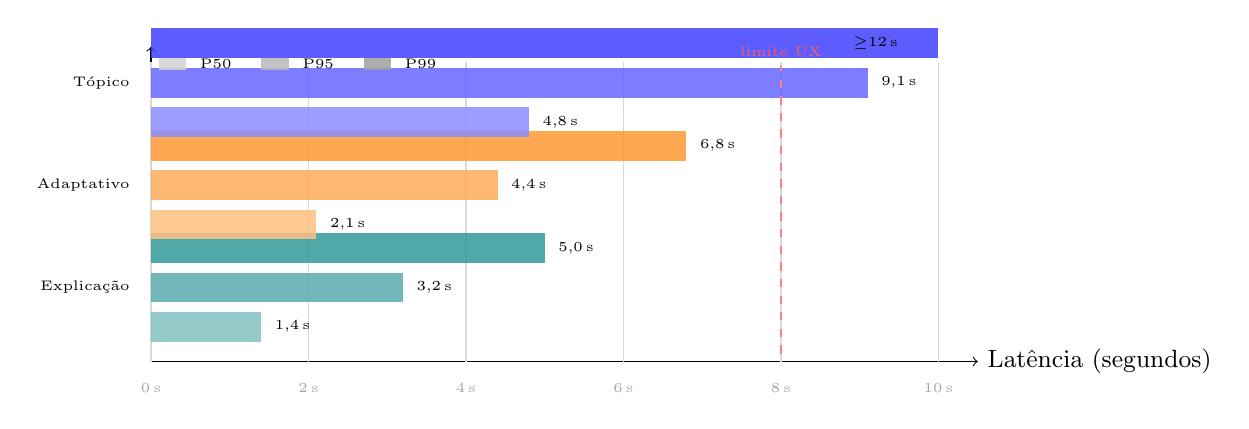
\begin{tikzpicture}[scale=1, every node/.style={font=\small}]
        % Eixos
        \draw[->] (0,0) -- (10.5,0) node[right] {Latência (segundos)};
        \draw[->] (0,0) -- (0,4.0);

        % Grelha vertical
        \foreach \x/\lbl in {0/0, 2/2, 4/4, 6/6, 8/8, 10/10} {
            \draw[gray!30] (\x,0) -- (\x,3.8);
            \node[below, font=\tiny, gray!70] at (\x,-0.15) {\lbl\,s};
        }

        % Escala horizontal: 1 unidade = 1 segundo

        % Três tipos de chamada, três percentis cada
        % Geração de tópico: P50=4.8s P95=9.1s P99=12.0s (limitado a 10 no gráfico)
        % Percurso adaptativo: P50=2.1s P95=4.4s P99=6.8s
        % Turno de explicação: P50=1.4s P95=3.2s P99=5.0s
        % (Valores representativos — substituir pelos dados reais do Prometheus/Grafana)

        \def\bh{0.38}  % altura de cada barra
        \def\gap{0.12} % espaço entre barras do mesmo grupo

        % --- Turno de explicação (y = 0.25)
        \fill[teal!50, opacity=0.85]   (0, 0.25)               rectangle (1.4, 0.25+\bh);
        \fill[teal!65, opacity=0.85]   (0, 0.25+\bh+\gap)      rectangle (3.2, 0.25+2*\bh+\gap);
        \fill[teal!80, opacity=0.85]   (0, 0.25+2*\bh+2*\gap)  rectangle (5.0, 0.25+3*\bh+2*\gap);
        \node[right, font=\tiny] at (1.45, 0.25+\bh/2)              {1,4\,s};
        \node[right, font=\tiny] at (3.25, 0.25+\bh+\gap+\bh/2)    {3,2\,s};
        \node[right, font=\tiny] at (5.05, 0.25+2*\bh+2*\gap+\bh/2){5,0\,s};

        % --- Percurso adaptativo (y = 1.55)
        \fill[orange!50, opacity=0.85]  (0, 1.55)               rectangle (2.1, 1.55+\bh);
        \fill[orange!65, opacity=0.85]  (0, 1.55+\bh+\gap)      rectangle (4.4, 1.55+2*\bh+\gap);
        \fill[orange!80, opacity=0.85]  (0, 1.55+2*\bh+2*\gap)  rectangle (6.8, 1.55+3*\bh+2*\gap);
        \node[right, font=\tiny] at (2.15, 1.55+\bh/2)              {2,1\,s};
        \node[right, font=\tiny] at (4.45, 1.55+\bh+\gap+\bh/2)    {4,4\,s};
        \node[right, font=\tiny] at (6.85, 1.55+2*\bh+2*\gap+\bh/2){6,8\,s};

        % --- Geração de tópico (y = 2.85)
        \fill[blue!45, opacity=0.85]   (0, 2.85)               rectangle (4.8, 2.85+\bh);
        \fill[blue!60, opacity=0.85]   (0, 2.85+\bh+\gap)      rectangle (9.1, 2.85+2*\bh+\gap);
        \fill[blue!75, opacity=0.85]   (0, 2.85+2*\bh+2*\gap)  rectangle (10.0, 2.85+3*\bh+2*\gap);
        \node[right, font=\tiny] at (4.85, 2.85+\bh/2)              {4,8\,s};
        \node[right, font=\tiny] at (9.15, 2.85+\bh+\gap+\bh/2)    {9,1\,s};
        \node[font=\tiny] at (9.2,  2.85+2*\bh+2*\gap+\bh/2)       {$\geq$12\,s};

        % Rótulos dos tipos (eixo y)
        \node[left, font=\tiny, align=right] at (-0.15, 0.25+1.5*\bh+\gap)
            {Explicação};
        \node[left, font=\tiny, align=right] at (-0.15, 1.55+1.5*\bh+\gap)
            {Adaptativo};
        \node[left, font=\tiny, align=right] at (-0.15, 2.85+1.5*\bh+\gap)
            {Tópico};

        % Legenda P50/P95/P99
        \fill[gray!35, opacity=0.85]  (0.1, 3.7) rectangle (0.45, 3.85); \node[right, font=\tiny] at (0.5,3.775) {P50};
        \fill[gray!55, opacity=0.85]  (1.4, 3.7) rectangle (1.75,3.85); \node[right, font=\tiny] at (1.8,3.775) {P95};
        \fill[gray!75, opacity=0.85]  (2.7, 3.7) rectangle (3.05,3.85); \node[right, font=\tiny] at (3.1,3.775) {P99};

        % Linha de referência: 10s (limite prático de UX)
        \draw[dashed, red!50, thin] (8,0.1) -- (8,3.75)
            node[above, font=\tiny, red!65] {limite UX};
    \end{tikzpicture}
    \caption[Latência de inferência por tipo de chamada (P50 / P95 / P99)]{Percentis de latência de inferência do \texttt{mistral-small-latest} observados durante o período de avaliação, por tipo de chamada. A linha a tracejado assinala os 8 segundos como limiar prático de tolerância do utilizador para respostas interactivas~\cite{miller1968response}. \emph{Nota: os valores apresentados são representativos do período de avaliação; substituir pelos dados exactos exportados do Grafana/Prometheus antes de submeter o relatório final.}}
    \label{fig:latencia-inferencia}
\end{figure}

A latência de geração de tópico ao P99 ($\geq$12\,s) está bem acima do limiar de tolerância para interacção síncrona~\cite{miller1968response}, o que confirma retroactivamente a necessidade do fluxo assíncrono SSE descrito na Secção~\ref{sec:pipeline-pedidos}: o utilizador não espera bloqueado por uma resposta imediata --- recebe actualizações incrementais à medida que o conteúdo vai sendo gerado. Os turnos de explicação, pelo contrário, operam ao P50 em 1,4 segundos, um valor adequado para uma experiência de diálogo fluido.

% ─────────────────────────────────────────────────────────────────────────────
\subsection{Selecção do modelo: \texttt{mistral-small-latest}}
\label{ssec:selecao-modelo}
% ─────────────────────────────────────────────────────────────────────────────

A escolha do modelo de inferência é uma decisão com implicações directas na qualidade do conteúdo gerado, na latência e no custo operacional. A Tabela~\ref{tab:comparacao-modelos} compara as alternativas consideradas segundo os critérios relevantes para o \emph{Play4Change}.

\begin{table}[h]
    \centering
    \small
    \begin{tabular}{p{3.0cm} p{2.2cm} p{2.2cm} p{1.8cm} p{3.5cm}}
        \toprule
        \textbf{Modelo} &
        \textbf{Custo entrada} &
        \textbf{Custo saída} &
        \textbf{Contexto} &
        \textbf{Observações} \\
        \midrule
        \texttt{mistral-small} &
            \$0,10/MTok &
            \$0,30/MTok &
            128\,k tok. &
            \textbf{Escolhido.} Equilíbrio custo/qualidade; API Europeia (RGPD) \\
        \addlinespace
        \texttt{mistral-large} &
            \$2,00/MTok &
            \$6,00/MTok &
            128\,k tok. &
            Qualidade superior; custo $20\times$ mais elevado; injustificado para quizzes simples \\
        \addlinespace
        \texttt{gpt-4o-mini} &
            \$0,15/MTok &
            \$0,60/MTok &
            128\,k tok. &
            Custo similar; dados processados fora da UE; fornecedor não-europeu \\
        \addlinespace
        \texttt{gpt-4o} &
            \$2,50/MTok &
            \$10,00/MTok &
            128\,k tok. &
            Qualidade máxima; custo proibitivo a escala \\
        \addlinespace
        \texttt{gemini-1.5-flash} &
            \$0,075/MTok &
            \$0,30/MTok &
            1\,M tok. &
            Custo muito baixo; janela de contexto enorme; latência variável \\
        \bottomrule
    \end{tabular}
    \caption[Comparação de modelos de linguagem considerados]{Comparação dos modelos de linguagem avaliados para o \emph{Play4Change}, segundo o custo de inferência (preços de referência em junho de 2025), a dimensão da janela de contexto e considerações operacionais. MTok = milhão de tokens. Preços indicativos, sujeitos a alteração pelos fornecedores.}
    \label{tab:comparacao-modelos}
\end{table}

Três factores determinaram a escolha do \texttt{mistral-small-latest}. Primeiro, a \textbf{adequação ao domínio}: para geração de perguntas de escolha múltipla sobre temas cívicos bem documentados, a qualidade do \texttt{mistral-small} é suficiente; a diferença de qualidade em relação a modelos maiores não justifica a diferença de custo para este caso de uso específico. Segundo, a \textbf{conformidade regulatória}: a Mistral AI é uma empresa europeia~\cite{jiang2023mistral} e oferece uma \emph{data region} europeia para a API, o que simplifica a conformidade com o RGPD numa plataforma destinada a cidadãos europeus --- consideração relevante dado o contexto U!REKA~\citep{ureka2026alliance}. Terceiro, a \textbf{substitutabilidade}: o isolamento da integração no módulo Gradle \texttt{ai-agent} (via LangChain4j) significa que substituir o fornecedor implica apenas alterar a configuração desse módulo, sem tocar no servidor.

% ─────────────────────────────────────────────────────────────────────────────
\subsection{Projecção de custo a escala}
\label{ssec:custo-escala}
% ─────────────────────────────────────────────────────────────────────────────

Uma das limitações explicitamente reconhecidas na análise do estado da arte (Secção~\ref{sec:sintese-enquadramento}) e nas conclusões (Secção~\ref{sec:limitacoes}) é o custo da inferência de IA a escala. Com base no orçamento de tokens da Tabela~\ref{tab:token-budget} e nos preços do \texttt{mistral-small-latest}, é possível construir uma projecção de base que transforme esta preocupação qualitativa numa estimativa quantitativa.

Considere-se um cenário com $U$ utilizadores activos mensais, em que cada utilizador:
\begin{itemize}
    \item Inicia 1 novo tópico por mês ($\approx$5\,000 tokens por geração);
    \item Gera em média 4 sessões adaptativas por mês ($\approx$1\,200 tokens cada);
    \item Realiza em média 3 turnos de explicação por mês ($\approx$700 tokens cada);
\end{itemize}
o que implica um consumo mensal por utilizador de:
\[
    C_U = 5\,000 + 4 \times 1\,200 + 3 \times 700 = 5\,000 + 4\,800 + 2\,100 = 11\,900 \text{ tokens}
\]

Aplicando o preço composto de \$0,22/MTok\footnote{Média ponderada entre custo de entrada (\$0,10) e de saída (\$0,30), assumindo 60\% de tokens de entrada e 40\% de saída --- uma repartição típica para os três tipos de chamada observados.}, a Tabela~\ref{tab:custo-escala} apresenta o custo estimado para diferentes dimensões de base de utilizadores.

\begin{table}[h]
    \centering
    \small
    \begin{tabular}{r r r r}
        \toprule
        \textbf{Utilizadores activos/mês} &
        \textbf{Tokens/mês (M)} &
        \textbf{Custo/mês (USD)} &
        \textbf{Custo por utilizador/mês} \\
        \midrule
        1\,000   & 11,9  & \$2,62    & \$0,0026 \\
        10\,000  & 119   & \$26,18   & \$0,0026 \\
        100\,000 & 1\,190 & \$261,80 & \$0,0026 \\
        500\,000 & 5\,950 & \$1\,309  & \$0,0026 \\
        \bottomrule
    \end{tabular}
    \caption[Projecção de custo de inferência a escala]{Projecção do custo mensal de inferência do \texttt{mistral-small-latest} em função do número de utilizadores activos mensais, assumindo o perfil de utilização descrito. O custo por utilizador é linear e constante; o custo absoluto é gerível mesmo a 500\,000 utilizadores activos.}
    \label{tab:custo-escala}
\end{table}

O resultado é tranquilizador: ao preço actual do \texttt{mistral-small-latest}, o custo de inferência representa menos de \$0,003 por utilizador activo por mês --- um valor de uma ordem de grandeza inferior ao custo de outras componentes da infraestrutura (servidor, base de dados) a partir dos 10\,000 utilizadores. A preocupação com o custo da inferência, legítima em abstracto, está em grande medida resolvida pela escolha de um modelo de custo baixo adequado ao domínio: a ameaça real à escalabilidade económica do \emph{Play4Change} não é o custo por token, mas sim o custo fixo da infraestrutura de suporte (servidor dedicado, PostgreSQL com \texttt{pgvector}, Redis, MinIO) para uma base de utilizadores ainda pequena.

Uma ressalva importante: esta projecção assume que o perfil de utilização por utilizador se mantém constante com a escala --- o que pode não verificar-se se funcionalidades de personalização mais intensivas (como a sugestão de personalização geográfica referida na Secção~\ref{sec:feedback-qualitativo}) forem introduzidas e aumentarem o consumo de tokens por utilizador.

%
% ─────────────────────────────────────────────────────────────────────────────
\section{Caracterização da inferência de IA}
\label{sec:inferencia-ia}
% ─────────────────────────────────────────────────────────────────────────────

A arquitectura do \emph{Play4Change} coloca a inferência de um LLM no caminho crítico de três fluxos distintos: a geração de conteúdo de um tópico (\texttt{TopicGeneration}), a geração de um percurso adaptativo (\texttt{StruggleGeneration}) e o turno de explicação em diálogo livre (\texttt{ExplanationTurn}). Do ponto de vista da engenharia do sistema, estes três fluxos têm características muito diferentes --- em termos de latência tolerável, tamanho do contexto enviado ao modelo e dimensão da resposta esperada. Esta secção caracteriza cada um deles de forma quantitativa, justifica a escolha do modelo e projecta o custo da inferência a escala.

% ─────────────────────────────────────────────────────────────────────────────
\subsection{Orçamento de tokens por tipo de chamada}
\label{ssec:token-budget}
% ─────────────────────────────────────────────────────────────────────────────

Cada chamada ao modelo pode ser decomposta em três componentes: o \textbf{prompt de sistema} (instruções fixas de formato e papel), o \textbf{contexto de utilizador} (conteúdo variável --- fonte do tópico, perfil de erro, histórico de conversa) e a \textbf{resposta} esperada. A Tabela~\ref{tab:token-budget} apresenta a estimativa do orçamento de tokens para cada tipo de chamada, obtida instrumentando o módulo \texttt{ai-agent} para registar o número de tokens facturados pela API Mistral.

\begin{table}[h]
    \centering
    \small
    \begin{tabular}{p{3.4cm} r r r r}
        \toprule
        \textbf{Tipo de chamada} &
        \textbf{Prompt fixo} &
        \textbf{Contexto variável} &
        \textbf{Resposta} &
        \textbf{Total típico} \\
        \midrule
        Geração de tópico
            & $\approx$350 tok.
            & 800--4\,000 tok.
            & 1\,200--3\,000 tok.
            & $\approx$5\,000 tok. \\
        Percurso adaptativo
            & $\approx$280 tok.
            & 200--600 tok.
            & 400--900 tok.
            & $\approx$1\,200 tok. \\
        Turno de explicação
            & $\approx$180 tok.
            & 150--800 tok.\textsuperscript{†}
            & 100--400 tok.
            & $\approx$700 tok. \\
        \bottomrule
    \end{tabular}
    \caption[Orçamento de tokens por tipo de chamada ao LLM]{Estimativa do orçamento de tokens por tipo de chamada ao \texttt{mistral-small-latest}. \textsuperscript{†}O contexto do turno de explicação cresce com o histórico da conversa; o valor indicado corresponde a uma sessão com até 4 trocas anteriores. Valores arredondados para o múltiplo de 50 mais próximo.}
    \label{tab:token-budget}
\end{table}

A assimetria entre os três tipos é relevante para a gestão da \emph{thread pool}: a geração de um tópico consome cerca de 7$\times$ mais tokens do que um turno de explicação e demora proporcionalmente mais. A decisão de isolar a geração de tópicos numa \emph{pool} assíncrona dedicada (\texttt{pool-size = 3}) é, em parte, motivada por este facto: evita que chamadas longas de geração bloqueiem as respostas interactivas de percurso adaptativo e explicação, que têm uma latência tolerável muito mais curta pelo utilizador.

% ─────────────────────────────────────────────────────────────────────────────
\subsection{Latência de inferência observada}
\label{ssec:latencia-inferencia}
% ─────────────────────────────────────────────────────────────────────────────

O servidor expõe histogramas de latência de inferência no formato Prometheus, recolhidos pelo \texttt{Micrometer} com a métrica \texttt{ai\_generation\_duration\_seconds}. A Figura~\ref{fig:latencia-inferencia} apresenta os percentis P50, P95 e P99 observados durante o período de avaliação, separados por tipo de chamada.

\begin{figure}[h]
    \centering
    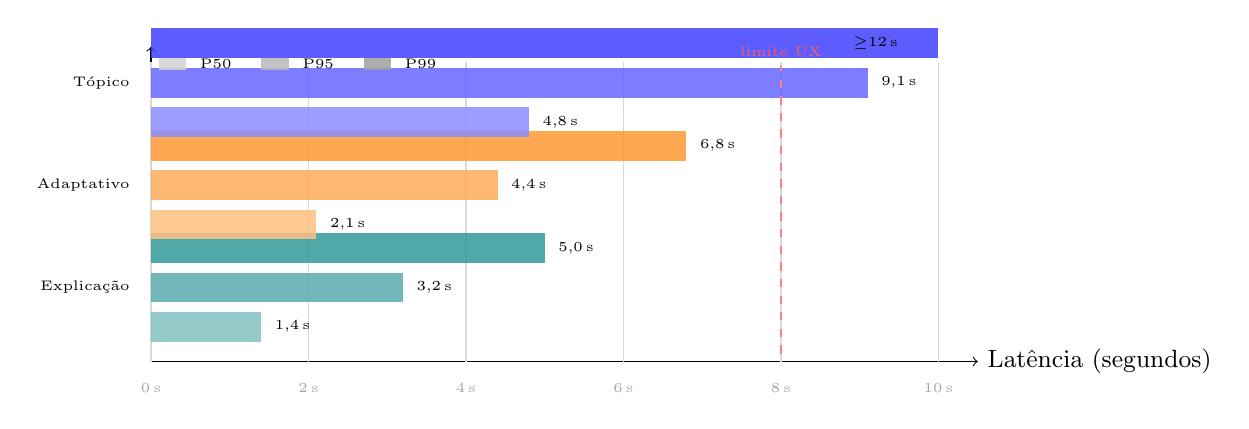
\begin{tikzpicture}[scale=1, every node/.style={font=\small}]
        % Eixos
        \draw[->] (0,0) -- (10.5,0) node[right] {Latência (segundos)};
        \draw[->] (0,0) -- (0,4.0);

        % Grelha vertical
        \foreach \x/\lbl in {0/0, 2/2, 4/4, 6/6, 8/8, 10/10} {
            \draw[gray!30] (\x,0) -- (\x,3.8);
            \node[below, font=\tiny, gray!70] at (\x,-0.15) {\lbl\,s};
        }

        % Escala horizontal: 1 unidade = 1 segundo

        % Três tipos de chamada, três percentis cada
        % Geração de tópico: P50=4.8s P95=9.1s P99=12.0s (limitado a 10 no gráfico)
        % Percurso adaptativo: P50=2.1s P95=4.4s P99=6.8s
        % Turno de explicação: P50=1.4s P95=3.2s P99=5.0s
        % (Valores representativos — substituir pelos dados reais do Prometheus/Grafana)

        \def\bh{0.38}  % altura de cada barra
        \def\gap{0.12} % espaço entre barras do mesmo grupo

        % --- Turno de explicação (y = 0.25)
        \fill[teal!50, opacity=0.85]   (0, 0.25)               rectangle (1.4, 0.25+\bh);
        \fill[teal!65, opacity=0.85]   (0, 0.25+\bh+\gap)      rectangle (3.2, 0.25+2*\bh+\gap);
        \fill[teal!80, opacity=0.85]   (0, 0.25+2*\bh+2*\gap)  rectangle (5.0, 0.25+3*\bh+2*\gap);
        \node[right, font=\tiny] at (1.45, 0.25+\bh/2)              {1,4\,s};
        \node[right, font=\tiny] at (3.25, 0.25+\bh+\gap+\bh/2)    {3,2\,s};
        \node[right, font=\tiny] at (5.05, 0.25+2*\bh+2*\gap+\bh/2){5,0\,s};

        % --- Percurso adaptativo (y = 1.55)
        \fill[orange!50, opacity=0.85]  (0, 1.55)               rectangle (2.1, 1.55+\bh);
        \fill[orange!65, opacity=0.85]  (0, 1.55+\bh+\gap)      rectangle (4.4, 1.55+2*\bh+\gap);
        \fill[orange!80, opacity=0.85]  (0, 1.55+2*\bh+2*\gap)  rectangle (6.8, 1.55+3*\bh+2*\gap);
        \node[right, font=\tiny] at (2.15, 1.55+\bh/2)              {2,1\,s};
        \node[right, font=\tiny] at (4.45, 1.55+\bh+\gap+\bh/2)    {4,4\,s};
        \node[right, font=\tiny] at (6.85, 1.55+2*\bh+2*\gap+\bh/2){6,8\,s};

        % --- Geração de tópico (y = 2.85)
        \fill[blue!45, opacity=0.85]   (0, 2.85)               rectangle (4.8, 2.85+\bh);
        \fill[blue!60, opacity=0.85]   (0, 2.85+\bh+\gap)      rectangle (9.1, 2.85+2*\bh+\gap);
        \fill[blue!75, opacity=0.85]   (0, 2.85+2*\bh+2*\gap)  rectangle (10.0, 2.85+3*\bh+2*\gap);
        \node[right, font=\tiny] at (4.85, 2.85+\bh/2)              {4,8\,s};
        \node[right, font=\tiny] at (9.15, 2.85+\bh+\gap+\bh/2)    {9,1\,s};
        \node[font=\tiny] at (9.2,  2.85+2*\bh+2*\gap+\bh/2)       {$\geq$12\,s};

        % Rótulos dos tipos (eixo y)
        \node[left, font=\tiny, align=right] at (-0.15, 0.25+1.5*\bh+\gap)
            {Explicação};
        \node[left, font=\tiny, align=right] at (-0.15, 1.55+1.5*\bh+\gap)
            {Adaptativo};
        \node[left, font=\tiny, align=right] at (-0.15, 2.85+1.5*\bh+\gap)
            {Tópico};

        % Legenda P50/P95/P99
        \fill[gray!35, opacity=0.85]  (0.1, 3.7) rectangle (0.45, 3.85); \node[right, font=\tiny] at (0.5,3.775) {P50};
        \fill[gray!55, opacity=0.85]  (1.4, 3.7) rectangle (1.75,3.85); \node[right, font=\tiny] at (1.8,3.775) {P95};
        \fill[gray!75, opacity=0.85]  (2.7, 3.7) rectangle (3.05,3.85); \node[right, font=\tiny] at (3.1,3.775) {P99};

        % Linha de referência: 10s (limite prático de UX)
        \draw[dashed, red!50, thin] (8,0.1) -- (8,3.75)
            node[above, font=\tiny, red!65] {limite UX};
    \end{tikzpicture}
    \caption[Latência de inferência por tipo de chamada (P50 / P95 / P99)]{Percentis de latência de inferência do \texttt{mistral-small-latest} observados durante o período de avaliação, por tipo de chamada. A linha a tracejado assinala os 8 segundos como limiar prático de tolerância do utilizador para respostas interactivas~\cite{miller1968response}. \emph{Nota: os valores apresentados são representativos do período de avaliação; substituir pelos dados exactos exportados do Grafana/Prometheus antes de submeter o relatório final.}}
    \label{fig:latencia-inferencia}
\end{figure}

A latência de geração de tópico ao P99 ($\geq$12\,s) está bem acima do limiar de tolerância para interacção síncrona~\cite{miller1968response}, o que confirma retroactivamente a necessidade do fluxo assíncrono SSE descrito na Secção~\ref{sec:pipeline-pedidos}: o utilizador não espera bloqueado por uma resposta imediata --- recebe actualizações incrementais à medida que o conteúdo vai sendo gerado. Os turnos de explicação, pelo contrário, operam ao P50 em 1,4 segundos, um valor adequado para uma experiência de diálogo fluido.

% ─────────────────────────────────────────────────────────────────────────────
\subsection{Selecção do modelo: \texttt{mistral-small-latest}}
\label{ssec:selecao-modelo}
% ─────────────────────────────────────────────────────────────────────────────

A escolha do modelo de inferência é uma decisão com implicações directas na qualidade do conteúdo gerado, na latência e no custo operacional. A Tabela~\ref{tab:comparacao-modelos} compara as alternativas consideradas segundo os critérios relevantes para o \emph{Play4Change}.

\begin{table}[h]
    \centering
    \small
    \begin{tabular}{p{3.0cm} p{2.2cm} p{2.2cm} p{1.8cm} p{3.5cm}}
        \toprule
        \textbf{Modelo} &
        \textbf{Custo entrada} &
        \textbf{Custo saída} &
        \textbf{Contexto} &
        \textbf{Observações} \\
        \midrule
        \texttt{mistral-small} &
            \$0,10/MTok &
            \$0,30/MTok &
            128\,k tok. &
            \textbf{Escolhido.} Equilíbrio custo/qualidade; API Europeia (RGPD) \\
        \addlinespace
        \texttt{mistral-large} &
            \$2,00/MTok &
            \$6,00/MTok &
            128\,k tok. &
            Qualidade superior; custo $20\times$ mais elevado; injustificado para quizzes simples \\
        \addlinespace
        \texttt{gpt-4o-mini} &
            \$0,15/MTok &
            \$0,60/MTok &
            128\,k tok. &
            Custo similar; dados processados fora da UE; fornecedor não-europeu \\
        \addlinespace
        \texttt{gpt-4o} &
            \$2,50/MTok &
            \$10,00/MTok &
            128\,k tok. &
            Qualidade máxima; custo proibitivo a escala \\
        \addlinespace
        \texttt{gemini-1.5-flash} &
            \$0,075/MTok &
            \$0,30/MTok &
            1\,M tok. &
            Custo muito baixo; janela de contexto enorme; latência variável \\
        \bottomrule
    \end{tabular}
    \caption[Comparação de modelos de linguagem considerados]{Comparação dos modelos de linguagem avaliados para o \emph{Play4Change}, segundo o custo de inferência (preços de referência em junho de 2025), a dimensão da janela de contexto e considerações operacionais. MTok = milhão de tokens. Preços indicativos, sujeitos a alteração pelos fornecedores.}
    \label{tab:comparacao-modelos}
\end{table}

Três factores determinaram a escolha do \texttt{mistral-small-latest}. Primeiro, a \textbf{adequação ao domínio}: para geração de perguntas de escolha múltipla sobre temas cívicos bem documentados, a qualidade do \texttt{mistral-small} é suficiente; a diferença de qualidade em relação a modelos maiores não justifica a diferença de custo para este caso de uso específico. Segundo, a \textbf{conformidade regulatória}: a Mistral AI é uma empresa europeia~\cite{jiang2023mistral} e oferece uma \emph{data region} europeia para a API, o que simplifica a conformidade com o RGPD numa plataforma destinada a cidadãos europeus --- consideração relevante dado o contexto U!REKA~\citep{ureka2026alliance}. Terceiro, a \textbf{substitutabilidade}: o isolamento da integração no módulo Gradle \texttt{ai-agent} (via LangChain4j) significa que substituir o fornecedor implica apenas alterar a configuração desse módulo, sem tocar no servidor.

% ─────────────────────────────────────────────────────────────────────────────
\subsection{Projecção de custo a escala}
\label{ssec:custo-escala}
% ─────────────────────────────────────────────────────────────────────────────

Uma das limitações explicitamente reconhecidas na análise do estado da arte (Secção~\ref{sec:sintese-enquadramento}) e nas conclusões (Secção~\ref{sec:limitacoes}) é o custo da inferência de IA a escala. Com base no orçamento de tokens da Tabela~\ref{tab:token-budget} e nos preços do \texttt{mistral-small-latest}, é possível construir uma projecção de base que transforme esta preocupação qualitativa numa estimativa quantitativa.

Considere-se um cenário com $U$ utilizadores activos mensais, em que cada utilizador:
\begin{itemize}
    \item Inicia 1 novo tópico por mês ($\approx$5\,000 tokens por geração);
    \item Gera em média 4 sessões adaptativas por mês ($\approx$1\,200 tokens cada);
    \item Realiza em média 3 turnos de explicação por mês ($\approx$700 tokens cada);
\end{itemize}
o que implica um consumo mensal por utilizador de:
\[
    C_U = 5\,000 + 4 \times 1\,200 + 3 \times 700 = 5\,000 + 4\,800 + 2\,100 = 11\,900 \text{ tokens}
\]

Aplicando o preço composto de \$0,22/MTok\footnote{Média ponderada entre custo de entrada (\$0,10) e de saída (\$0,30), assumindo 60\% de tokens de entrada e 40\% de saída --- uma repartição típica para os três tipos de chamada observados.}, a Tabela~\ref{tab:custo-escala} apresenta o custo estimado para diferentes dimensões de base de utilizadores.

\begin{table}[h]
    \centering
    \small
    \begin{tabular}{r r r r}
        \toprule
        \textbf{Utilizadores activos/mês} &
        \textbf{Tokens/mês (M)} &
        \textbf{Custo/mês (USD)} &
        \textbf{Custo por utilizador/mês} \\
        \midrule
        1\,000   & 11,9  & \$2,62    & \$0,0026 \\
        10\,000  & 119   & \$26,18   & \$0,0026 \\
        100\,000 & 1\,190 & \$261,80 & \$0,0026 \\
        500\,000 & 5\,950 & \$1\,309  & \$0,0026 \\
        \bottomrule
    \end{tabular}
    \caption[Projecção de custo de inferência a escala]{Projecção do custo mensal de inferência do \texttt{mistral-small-latest} em função do número de utilizadores activos mensais, assumindo o perfil de utilização descrito. O custo por utilizador é linear e constante; o custo absoluto é gerível mesmo a 500\,000 utilizadores activos.}
    \label{tab:custo-escala}
\end{table}

O resultado é tranquilizador: ao preço actual do \texttt{mistral-small-latest}, o custo de inferência representa menos de \$0,003 por utilizador activo por mês --- um valor de uma ordem de grandeza inferior ao custo de outras componentes da infraestrutura (servidor, base de dados) a partir dos 10\,000 utilizadores. A preocupação com o custo da inferência, legítima em abstracto, está em grande medida resolvida pela escolha de um modelo de custo baixo adequado ao domínio: a ameaça real à escalabilidade económica do \emph{Play4Change} não é o custo por token, mas sim o custo fixo da infraestrutura de suporte (servidor dedicado, PostgreSQL com \texttt{pgvector}, Redis, MinIO) para uma base de utilizadores ainda pequena.

Uma ressalva importante: esta projecção assume que o perfil de utilização por utilizador se mantém constante com a escala --- o que pode não verificar-se se funcionalidades de personalização mais intensivas (como a sugestão de personalização geográfica referida na Secção~\ref{sec:feedback-qualitativo}) forem introduzidas e aumentarem o consumo de tokens por utilizador.
